\chapter{Voigt Profile Fitting}  \label{chap:VPFIT}

\section{Voigt Profile}

The spectral lines are not infinitesimally peaked functions but rather have finite widths. This finite width or broadening can be attributed to the thermal motions of atoms (thermal broadening), quantum mechanical uncertainties in the energies of the transitions (natural broadening), collisions between excited atoms (collision broadening), etc. In astrophysical spectra the broadening is mainly thermal and natural broadening, the former results in Gaussian profile of the line whereas later gives a Lorentzian feature to the line profile. The convolution of these Gaussian and Lorentzian profiles results in what is known as the Voigt profile. The central region of an absorption line has a Gaussian shape whereas the extended wings show Lorentzian shape. So the absorption line in an astrophysical spectra can be modelled as Voigt profile. 
\\\\
The absorption profile at frequency $\nu$ can be written as:
\begin{equation*}
f(\nu)=f_{c} \ e^{-\tau(\nu)}
\end{equation*}
where $f, \ f_{c}, \ \tau$ are spectral flux density, interpolated absorption-free continuum over the absorption profile and optical depth respectively.

If we assume that the absorbing atoms have a Gaussian velocity distribution with mean velocity $v_0$ with respect to a reference frame, say S, then the optical depth is given by:

\begin{equation}  \label{eqn:tau}
\tau(\nu)=N \frac{1}{\sqrt{\pi}b}\int_{-\infty}^{\infty}\sigma(\nu')\ e^{-\frac{(v-v_0)^2}{b^2}} \text{d}v 
\end{equation}
where $N$ is the column density, $b$ is the Doppler parameter, which is defined as $b=FWHM/2\sqrt{ln2}$; $FWHM$ is the full width at half maximum and $\sigma(\nu')$ is the cross-section offered by an atom moving with the velocity $v$ to the photon of frequency $\nu$ in S and $\nu'=\nu/(1-v/c)$, taking $v$ to be positive for atoms receding away from the observer.  

The Doppler parameter $b$, has contributions from both thermal and non-thermal components (e.g. turbulence, etc.), which can be written as :
\begin{equation}
b=\sqrt{{b_{thermal}^2+b_{non-thermal}^2}}
\end{equation}
And $b_{thermal}$ is related to temperature (T) of the gas by $b_{thermal}=\sqrt{\frac{2kT}{m}}$, where $m$ is the mass of an atom and $k$ is the Boltzmann constant.
\\
We can get expression for cross-section in an atomic transition from the classical expression by taking in the factors of oscillator strength $(f)$ and frequency dependence which results from the finite life-time of the upper level of the transition. This expression is given by:
\begin{equation} \label{eqn:sigma}
\sigma=f \times \frac{1}{4\pi\epsilon_0} \frac{\pi e^2}{m_ec} \times \frac{1}{\pi} \frac{\frac{\gamma}{4\pi}}{{(\nu-\nu_0)}^2+{\frac{\gamma}{4\pi}}^2}
\end{equation}
where $\gamma$ is the total damping constant (de-excitation rate of the upper level) and other symbols have their usual meanings for the fundamental constants \citep{Voigt-eqn}. 
\\
Using equations \ref{eqn:sigma} \& \ref{eqn:tau} and changing frequency ($\nu$) to wavelength ($\lambda$) and putting values of the fundamental constants we get:

\begin{equation} \label{eqn:tau-lambda}
\tau(\lambda)=1.498 \times 10^{-2} \frac{Nf\lambda}{b} H(a,u)    
\end{equation}
where $H(a,u)$ is called the Voigt function and given as :
\begin{equation} \label{eqn:Voigt-func}
    H(a,u)=\frac{a}{\pi} \int_{-\infty}^{\infty} \frac{e^{-y^2}}{{(u-y)}^2+a^2} \text{d}y; \ a=\frac{\lambda \gamma}{4\pi b}; \ u=-\frac{c}{b}\left((1+\frac{v}{c})-\frac{\lambda}{\lambda_0}\right) 
\end{equation}
And $\lambda_0$ is the wavelength at the centre of the absorption profile. Clearly, the Voigt function is a convolution of gaussian and lorentizian functions. The absorption feature which is just $e^{-\tau(\lambda)}$, is called a Voigt profile.
\\\\
Figure \ref{fig:Voigt-b} shows simulated Voigt profile absorption lines with varying Doppler parameters at a fixed column density of $10^{13}$ cm$^{-2}$. It is evident from the figure \ref{fig:Voigt-b} that as the $b$ value increases the profile gets broader and shallower. So we require a very high S/N data to detect such shallow absorption features. Also, the optical depth at the center of the line decreases as $b$ increases. 

\begin{figure}[!h]
    \centering
    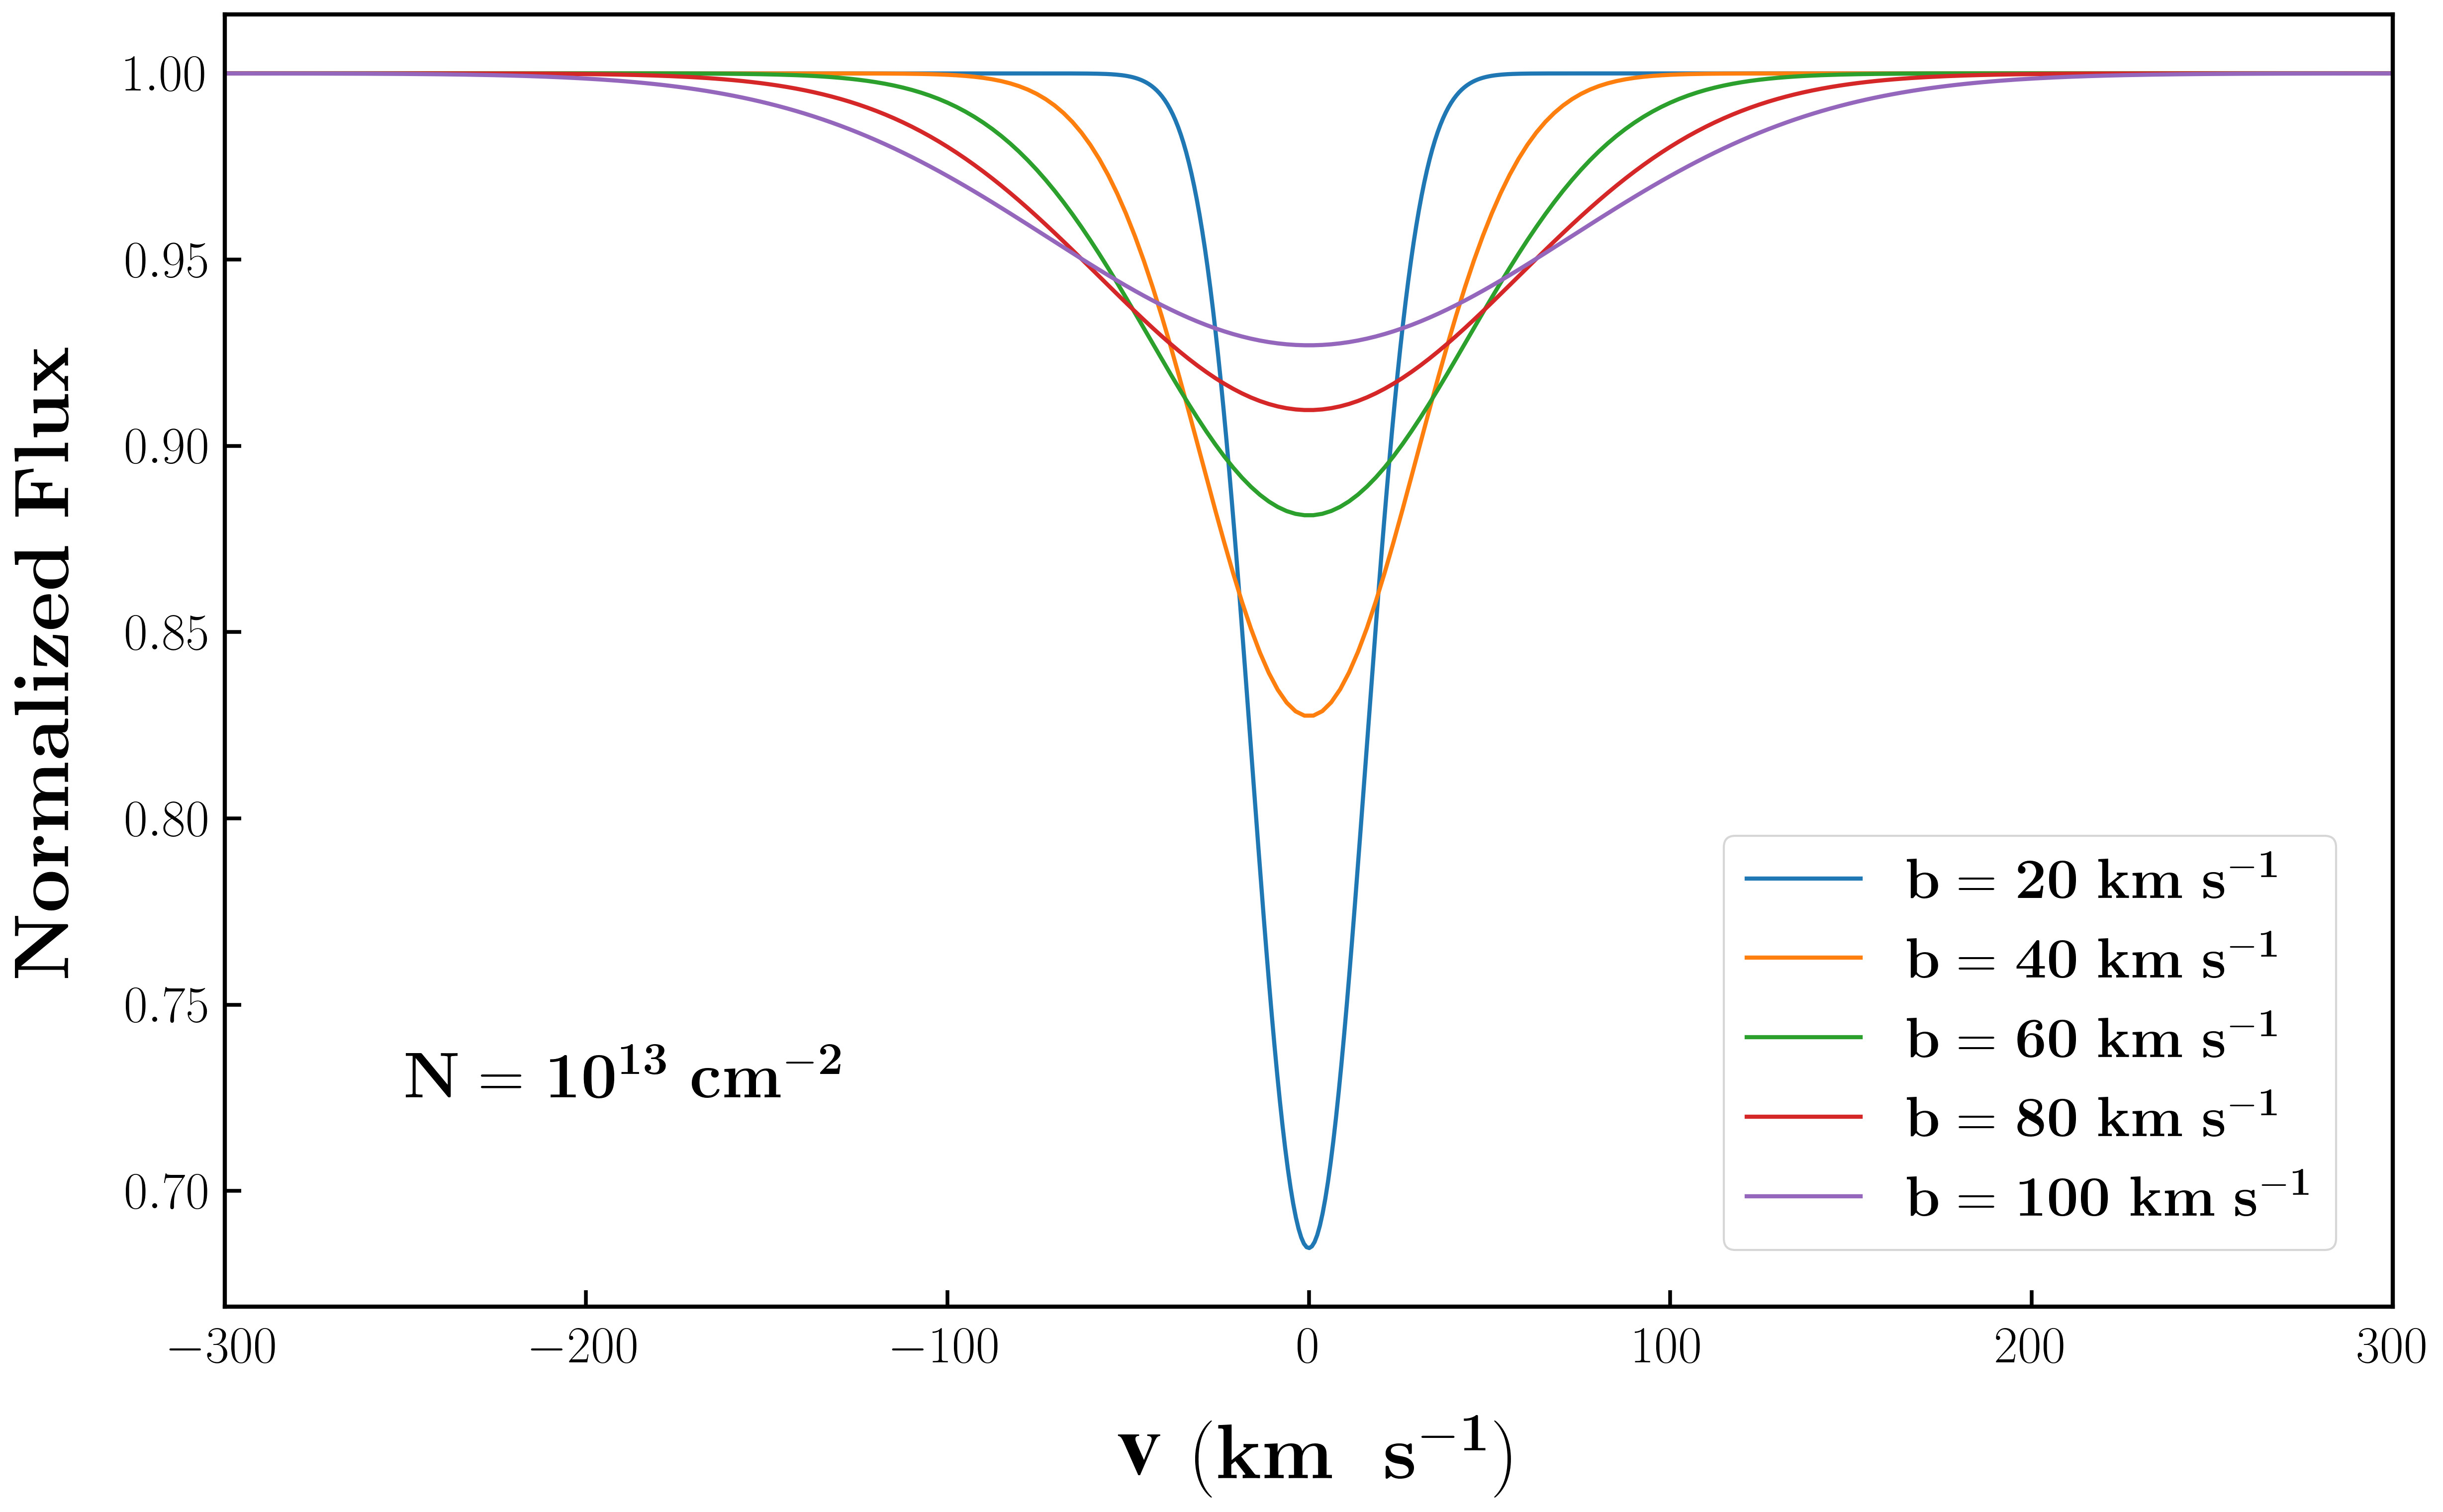
\includegraphics[width=\linewidth]{Figures/Voigt-b.jpg}
    \caption{Simulated Voigt profiles for different Doppler parameters. X-axis is the velocity from the central wavelength, taken as a proxy of wavelength}
    \label{fig:Voigt-b}
\end{figure}

Whereas figure \ref{fig:Voigt-N} shows the variation of Voigt absorption profile with column densities at a fixed Doppler parameter of 50 km s$^{-1}$. Now, as the column density increases, the optical depth at the center of the line increases resulting in the drop in flux, finally leading to the saturation of the profile, i.e. flux dropping to 0. Further increase in column density leads to the spread of profile and absorption from the wings also starts becoming prominent.

\begin{figure}[!t]
    \centering
    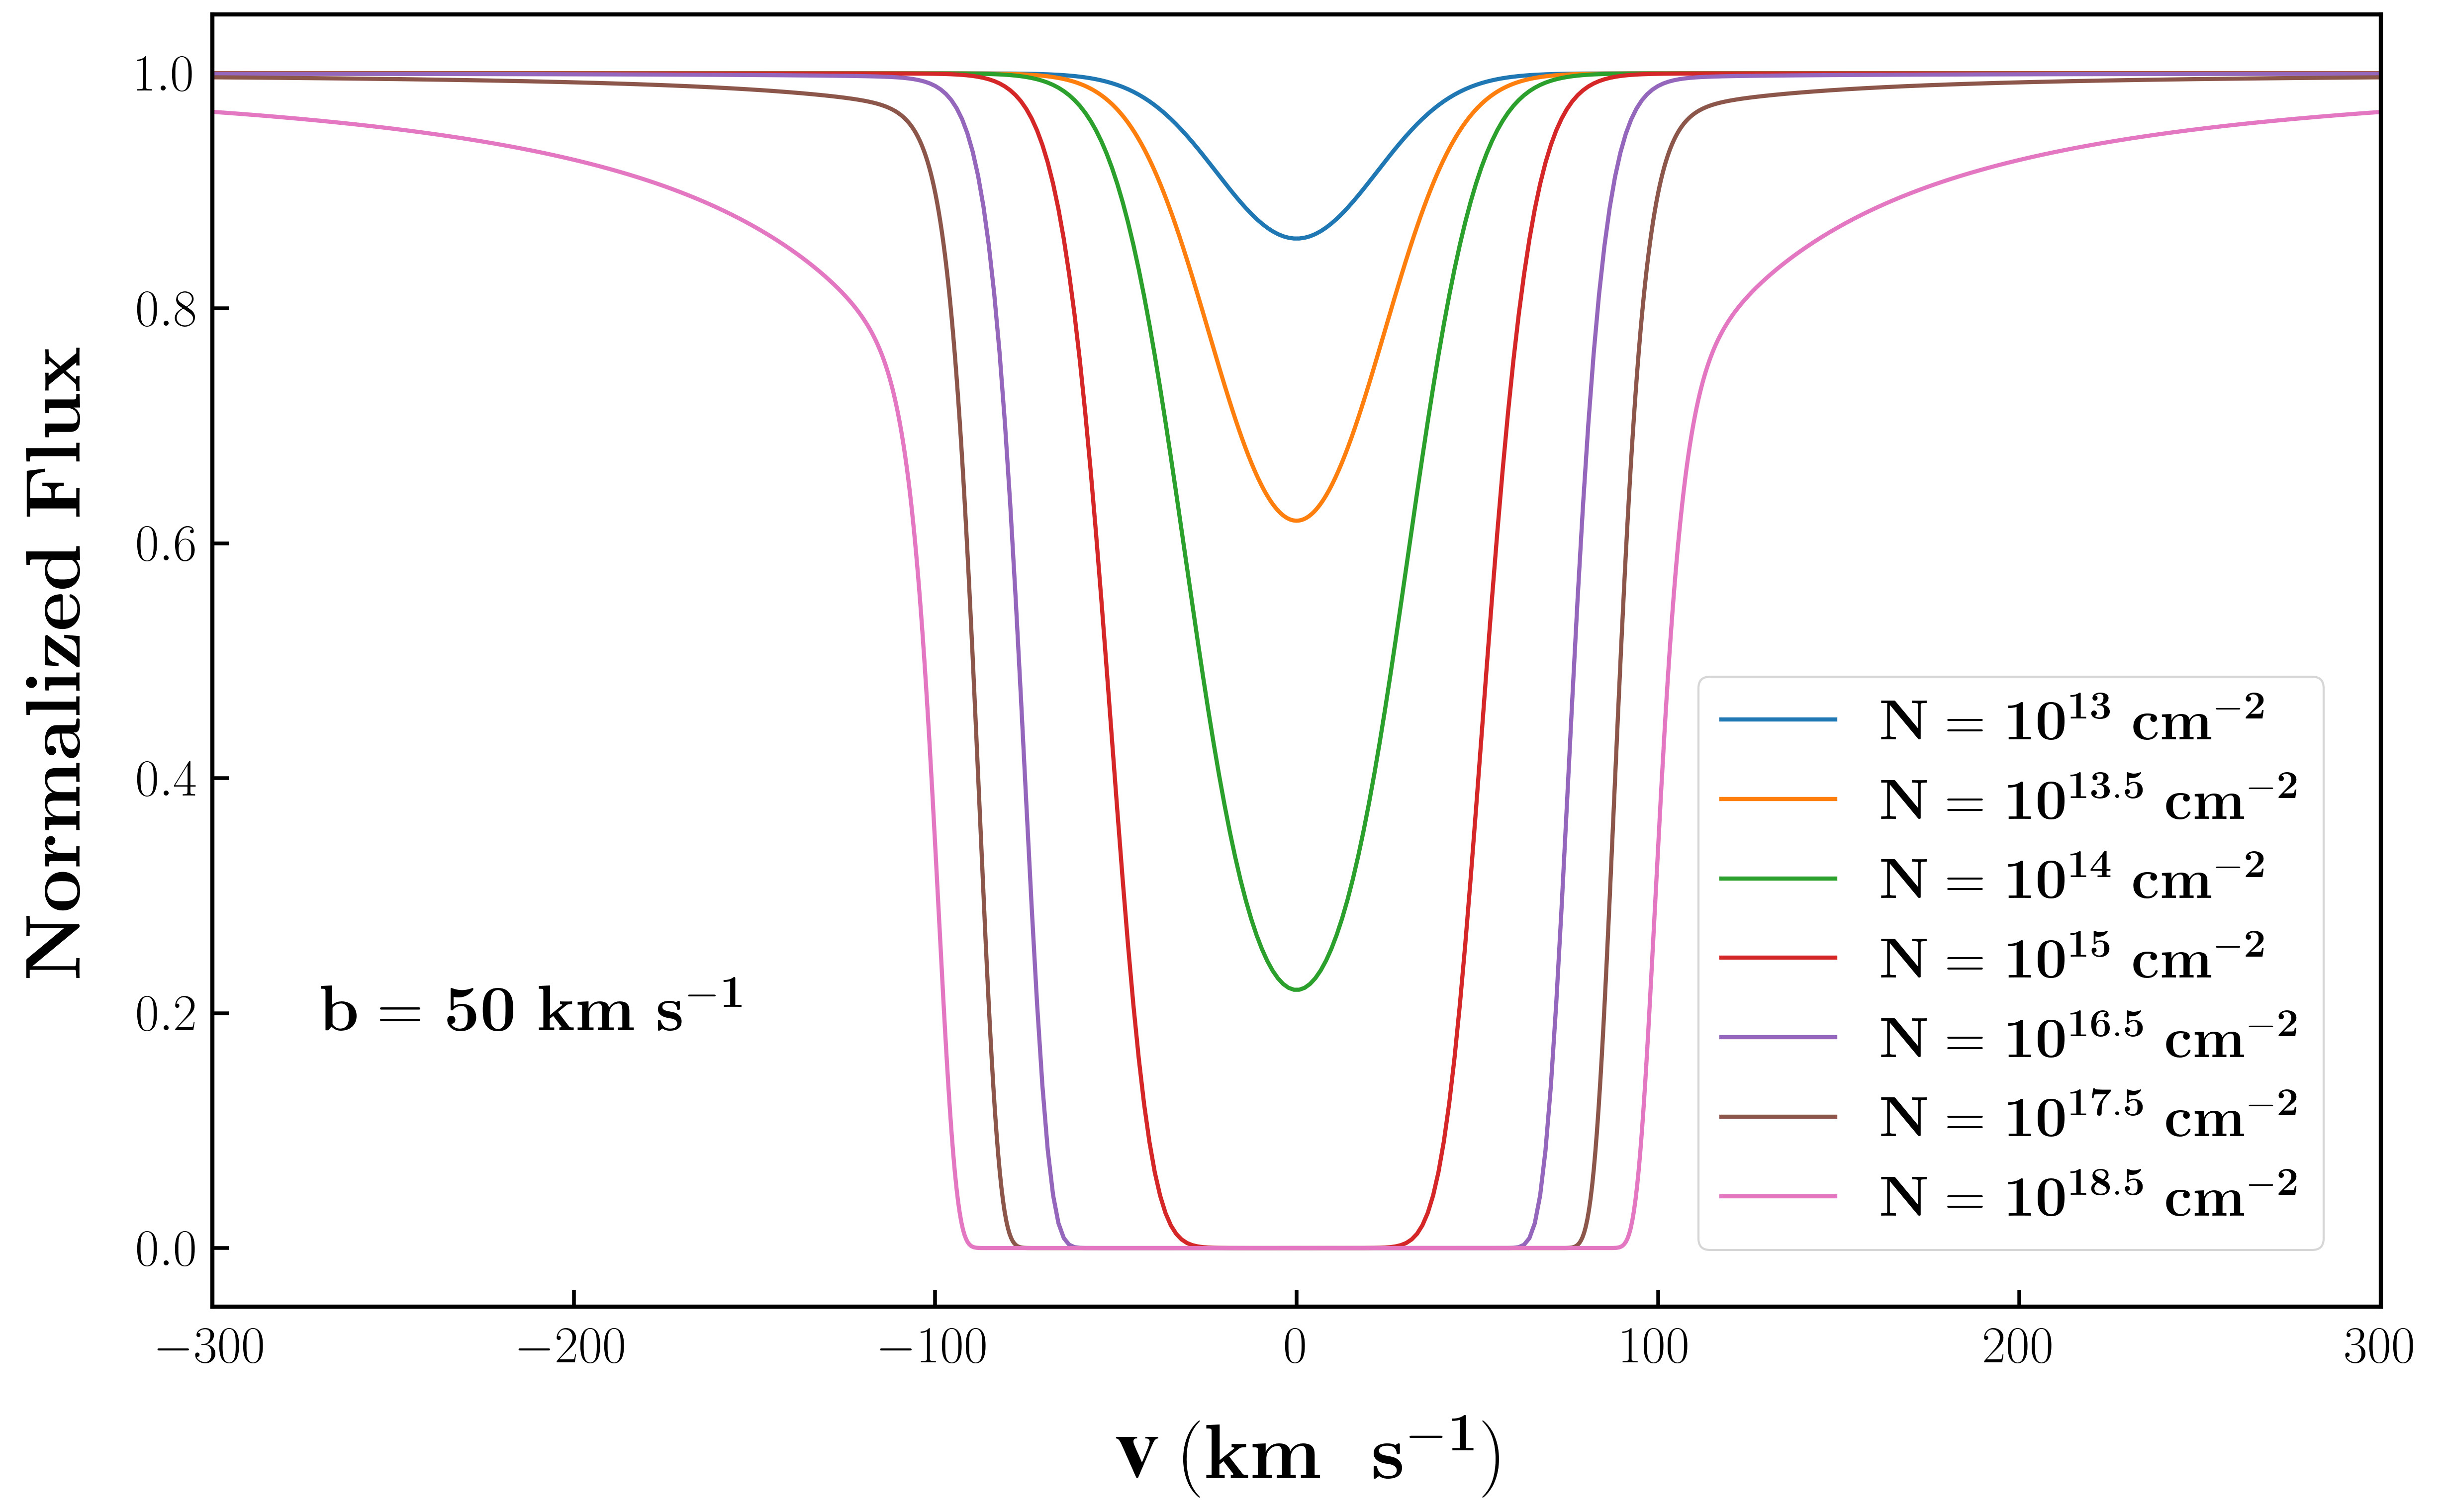
\includegraphics[width=\linewidth]{Figures/Voigt-N.jpg}
    \caption{Simulated Voigt profiles for different column densities. X-axis is the velocity from the central wavelength, taken as a proxy of wavelength}
    \label{fig:Voigt-N}
\end{figure}


\section{VPFIT}

Fitting Voigt profiles to the absorption lines in the spectrum of quasars is a very tedious task. The absorption lines can have the blend of multiple components of the same line or can be contaminated from some other line falling in the absorption profile of the line of interest. Furthermore, the atomic data characterising the transitions have to be carefully used.  All such challenges can't be solved using simple curve fitting tools available. 
\\\\
To fit the Voigt profiles to the absorption lines, we use Voigt profile fitting program ({\tt VPFIT}) \citep{vpfit}, which is developed specifically to deal with the absorption lines in astrophysical spectra . {\tt VPFIT} minimises the $\chi^2$ by varying the parameters in the parameter space. It gives 3 parameters and associated 1-$\sigma$ errors for each profile viz. redshift of the line (wavelength at centre of the absorption profile) , Doppler parameter (\emph{b}) and column density of the ion causing the absorption. We give {\tt VPFIT} an input file mentioning the continuum normalised spectrum, the wavelength region(s) to fit, initial guesses for the parameters and the ion for which we are fitting the absorption line. It also has a provision to include the instrument profiles in the form of line spread function (LSF) files. If LSF files are given, it then convolves the instrument profile and Voigt profiles. We use \textit{HST}/COS LSF files available on the STScI website\footnote{https://www.stsci.edu/hst/instrumentation/cos/performance/spectral-resolution}. In {\tt VPFIT}, we give the instrument profile as the LSF file of wavelength which lies between the fitting region of the line, if LSF file for such wavelengths is not available we then give the nearest wavelength LSF file available to the fitting region wavelengths. {\tt VPFIT} can also fit multiple Voigt profiles to the absorption lines in case multiple components are seen in the absorption lines. An example of Voigt profile fitting using {\tt VPFIT} is describe in section \ref{sec:VPfit-example}.

\subsection{Line-identification}

\citet{danforth-2016} have identified all the IGM absorber systems along each of the 82 lines of sight selected by them. They have also done the line identification of all the lines in each of the 82 spectra along with preliminary line fitting. However, their line fitting is not rigorous enough to be considered for our project as our results significantly depend on the line parameters. They have fitted the lines arising from same ions separately, leading to different parameters for the same ion. In principle, all the lines coming from a particular ion should be fitted simultaneously with same profiles, e.g. all the Lyman transitions should be fitted together rather than fitting Ly$\alpha$, Ly$\beta$, etc. alone. This helps us to better constrain the line parameters. For our fitting routine we use the line identification done by \citet{danforth-2016} and use their results as initial guess for our fitting procedure.

\vfill

\subsection{Example}  \label{sec:VPfit-example}

Figure \ref{fig:VPFIT-fit} shows an example of fitting a Voigt profile to an absorption line using {\tt VPFIT}. Figure \ref{fig:VPFIT-ip} gives the snapshot of an {\tt VPFIT} input file. In the first line we specify the continuum normalised spectrum (\emph{pks0405\_cont\_norm.asc}) and give a wavelength region where the profile is to be fitted in units used in the spectrum (\emph{1138.8 - 1141.4}) and we also give the LSF file as argument to \emph{pfinst}. In the considered example, we fit the line with two \ion{C}{iii} components by giving initial guesses of redshift (\emph{0.166588} \& \emph{0.167018}), Doppler parameter (\emph{39.7} \& \emph{35.3}) and column density (\emph{13.51} \& \emph{14.42})
 
The figure \ref{fig:VPFIT-op} shows the output file from {\tt VPFIT}. It gives us various statistics of the fit like number of iterations used (\emph{10}), reduced $\chi^2$ (\emph{1.380970}), etc. and the fitted line parameters and their 1$\sigma$ error.

It also displays the fit of the line as given in figure \ref{fig:VPFIT-fit}. The white step curve is the input spectrum and the green curve is the fitted Voigt profile. It shows that two components of \ion{C}{III} 977 line are fitted. It also allows us to save the fit in a separate file allowing further analysis on the data.


\begin{figure}[!htbp]
    \centering
     \begin{subfigure}[t]{\textwidth}
         \centering
         {
            \setlength{\fboxsep}{0pt}
            \setlength{\fboxrule}{1pt}
            \fbox{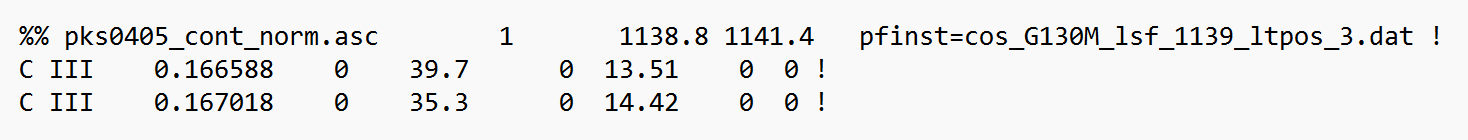
\includegraphics[width=\textwidth]{Figures/VPFIT_ip.png}}
}
         \caption{An example input file to {\tt VPFIT}}
         \label{fig:VPFIT-ip}
     \end{subfigure}

\medskip
\medskip
\medskip

    \begin{subfigure}[t]{\textwidth}
         \centering
         {
            \setlength{\fboxsep}{0pt}
            \setlength{\fboxrule}{1pt}
            \fbox{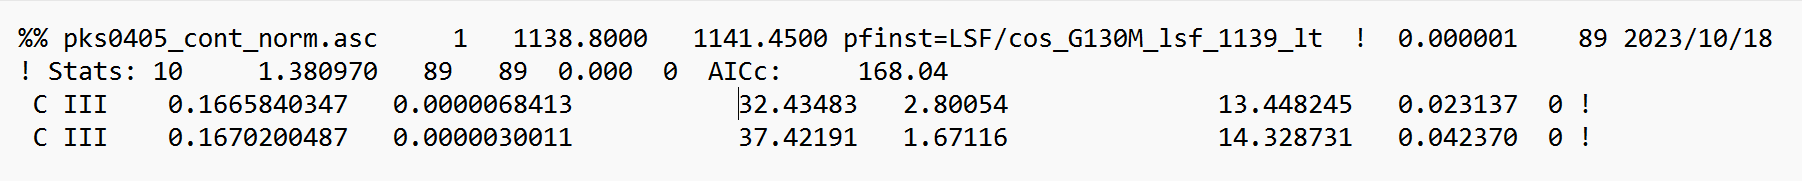
\includegraphics[width=\textwidth]{Figures/VPFIT_op.png}}
}
         \caption{An example output file from {\tt VPFIT}}
         \label{fig:VPFIT-op}
     \end{subfigure}
    \caption{Input to {\tt VPFIT} and output from {\tt VPFIT}}
    \label{fig:ip-op}
\end{figure}

\newpage

\begin{figure}[!t]
    % \vspace{-75mm}
     \centering
     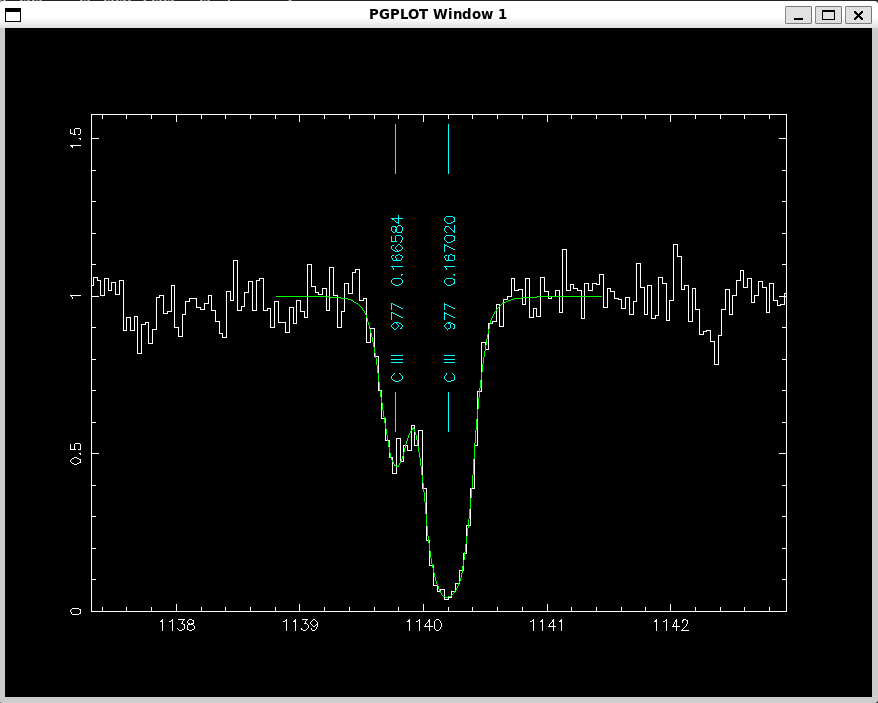
\includegraphics[width=0.8\textwidth]{Figures/VPFIT_fit.png}
     \caption{An example 2 component fit as displayed in {\tt VPFIT}}
     \label{fig:VPFIT-fit} 
\end{figure}

We use {\tt VPFIT} to fit the Voigt profiles to the absorption lines as described in this chapter. We use the column densities and Doppler parameters from Voigt profile fitting to model the ionisation conditions in the absorbers as described in next chapter.  